\documentclass[18pt]{article}
\usepackage[utf8]{inputenc}
\usepackage[T1]{fontenc}
\usepackage{ragged2e}
\usepackage{caladea}
\usepackage{graphicx}
\usepackage{longtable}
\usepackage{wrapfig}
\usepackage{rotating}
\usepackage{epigraph}
\usepackage[normalem]{ulem}
\usepackage{hyperref}
\usepackage{amsmath}
\usepackage{amssymb}
\usepackage{capt-of}
\usepackage{hyperref}
\usepackage{fancyhdr}

\title{
 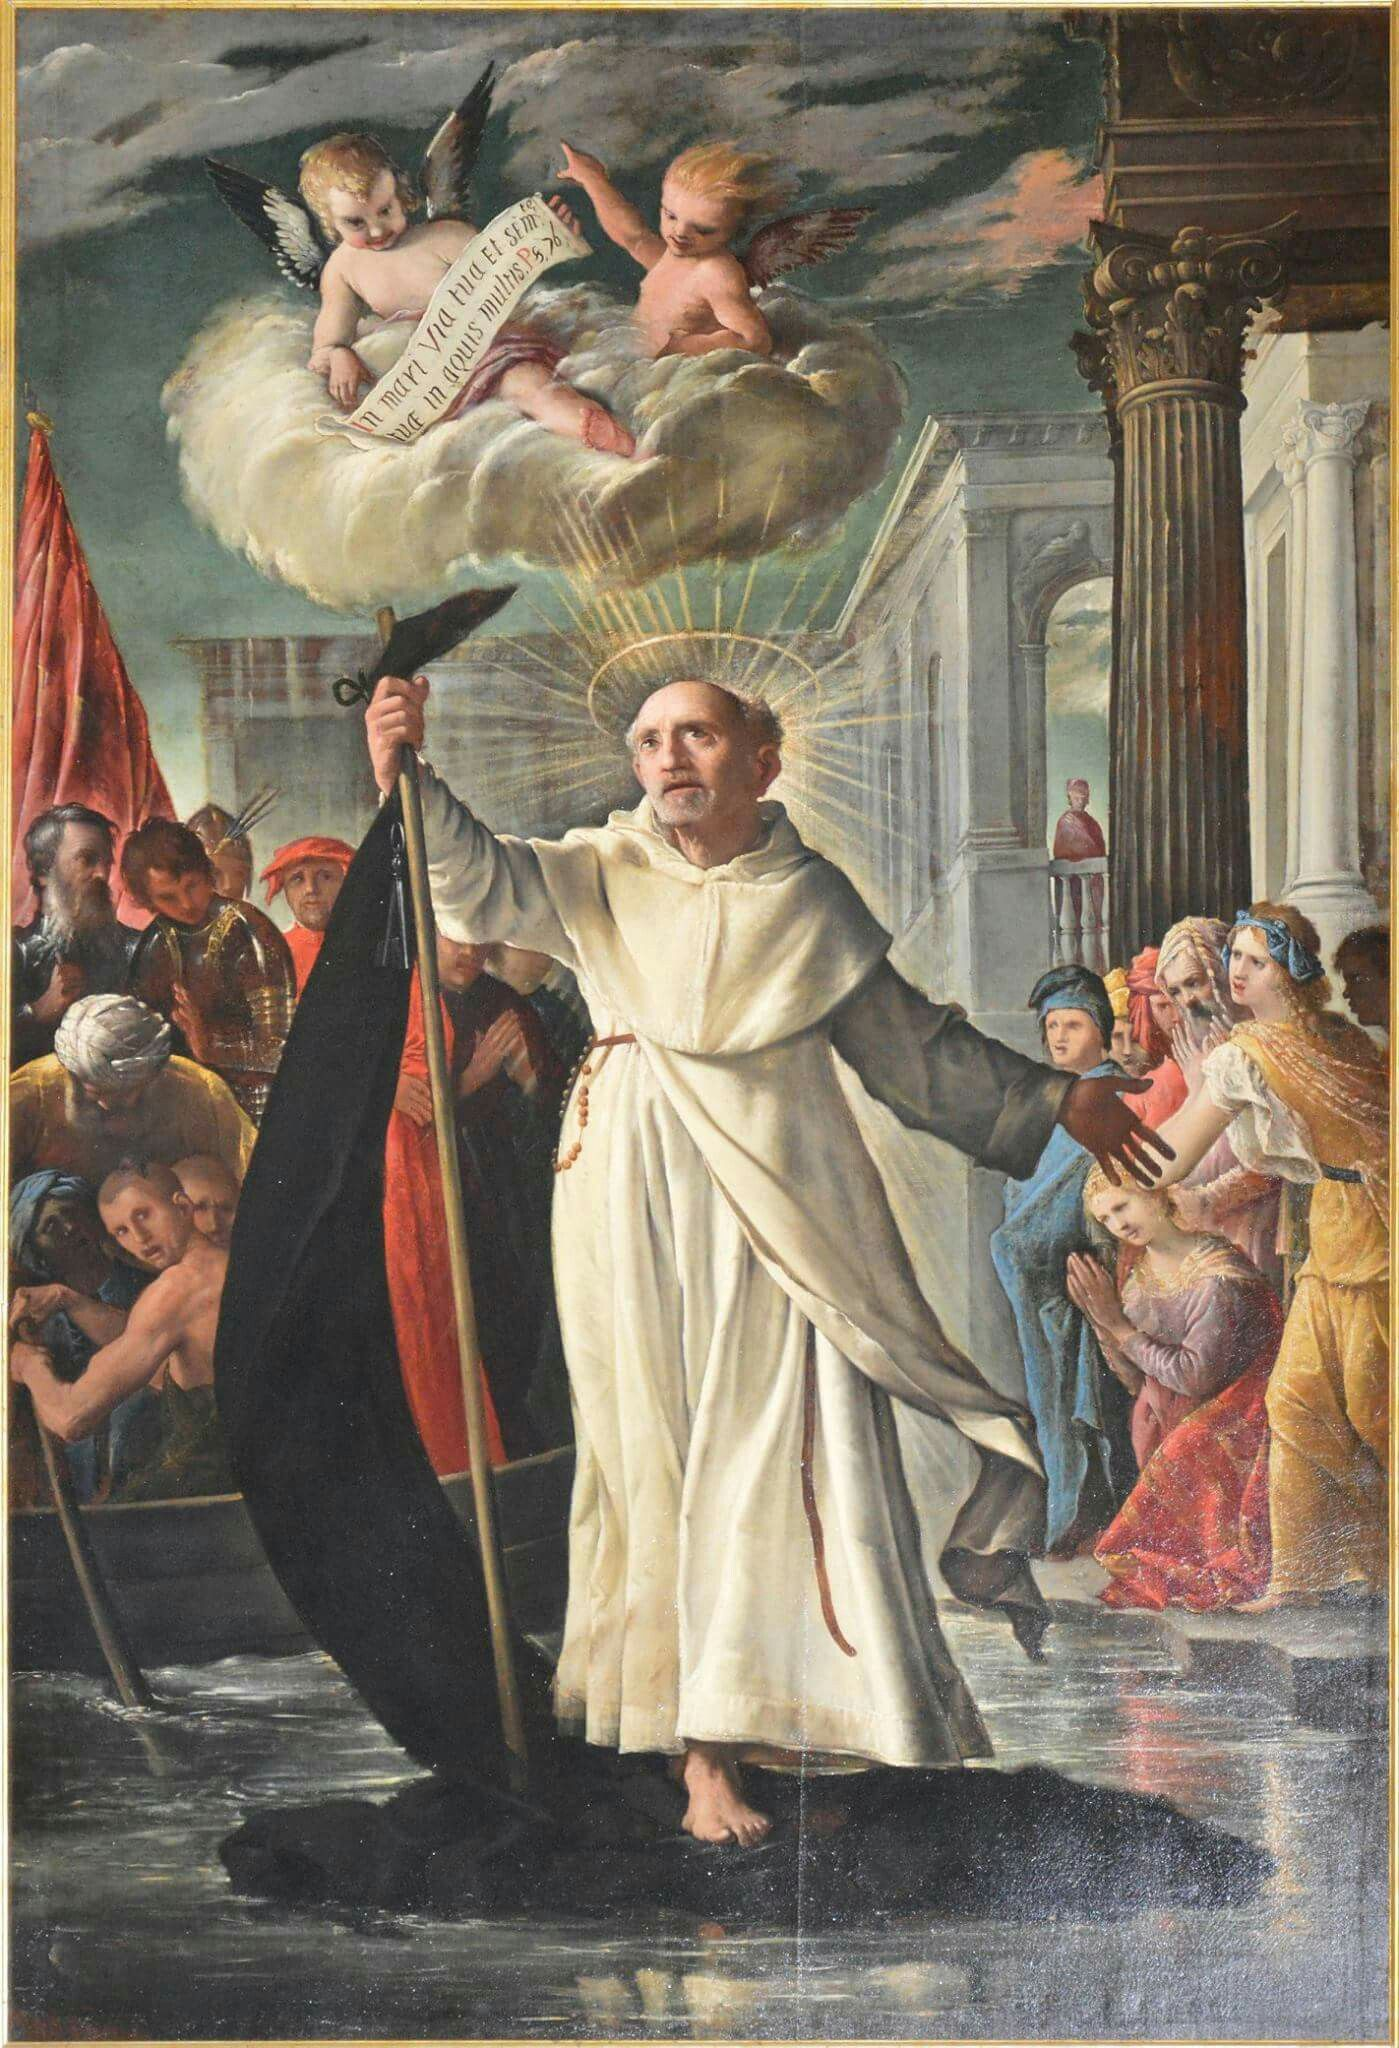
\includegraphics[scale=0.20, trim={10cm, 0, 10cm, 0}]{./assets/imagem.jpg}
  \par
   NOVENA A SÃO RAIMUNDO DE PENÃFORT}
\author{Garamog, Nina Freitas}
\date{Início da Novena: 29/12 - Data Litúrgica: 07/01 }

% Comando para fazer "Sumário" não aparecer no Sumário.
\renewcommand{\contentsname}{Sumário}
\begin{document}
\maketitle

\thispagestyle{empty} %zera a primeira página


\pagestyle{fancy}
\fancyhf{} % clear existing header/footer entries
\fancyfoot[LO, CE]{
  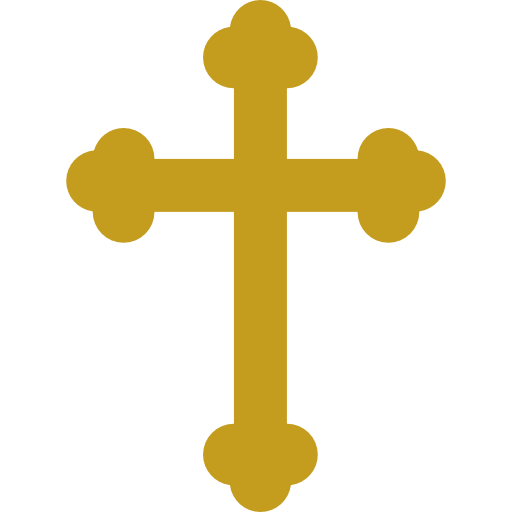
\includegraphics[scale=0.2]{./assets/cross.png} São Raimundo de Penãfort, rogai por nós!
}
% Place Page X of Y on the right-hand
% side of the footer
\fancyfoot[R]{\thepage}

\newpage

\tableofcontents

\centering
\vfill
Visite-nos no Telegram: \url{https://t.me/CotidieNovena}
\newpage

\newpage


\begin{justify}

 \begin{center}
  \section{História}\label{sec:História} % (fold)
 \end{center}


\subsection*{Origens}

São Raimundo nasceu no castelo de Peñafort, em Barcelona, Espanha, no ano de 1175. Seus pais originavam-se dos antigos condes de Barcelona e eram aliados do rei Aragão. Desde cedo, muito dedicado aos estudos, ele se especializou em Bolonha, na Itália, na universidade onde se tornou também um reconhecido mestre.

\subsection*{Entrada na Ordem Dominicana}

Deixou aquela realidade que tanto amava para obedecer ao Bispo de Barcelona, que o queria como cônego. Ele prestou esse serviço até discernir seu chamado à vida religiosa, foi quando entrou para a família dominicana e continuou em vários cargos de formação, mas aberto à realidade e às necessidades da Igreja, onde exerceu o papel de teólogo do Cardeal-bispo de Sabina; também foi legado na região de Castela e Aragão; depois, transferido para Roma, ocupou vários cargos.

\subsection*{Cúria Romana}

Ele não buscava nem tinha em mente um projeto de ocupar este ou aquele serviço, mas foi fiel àquilo que davam a ele como trabalho para a edificação da Igreja. Na Cúria Romana, quantos cargos ligados a Teologia, Direito Canônico. Um homem de prudência, de governo. Seu último cargo foi de penitenciário-mor do Sumo Pontífice. Quiseram até escolhê-lo como Arcebispo, mas, nesta altura, ele voltou para a Espanha; quis viver em seu convento, em Barcelona, como um simples frade, mas os reis, o Papa e tantos outros sempre recorriam ao seu discernimento.

\subsection*{Humilde homem}

São Raimundo escreveu a respeito da casuística. Enfim, pelos escritos e pelos ensinos, ele investia numa ação de mestres e missionários, pois tinha consciência de que precisava de missionários bem formados para que a evangelização também fluísse. Ele não fez nada sozinho, contou com a ajuda de São Tomás de Aquino, ajudou outros a discernir a vontade do Senhor, como São Pedro Nolasco, que estava discernindo a fundação de uma nova ordem consagrada a Nossa Senhora das Mercês – os mercedários. Homem humilde que se fez servo, foi escolhido como Superior Geral dos Dominicanos. Homem de pobreza, de obediência e pureza; homem de oração.

\subsection*{Páscoa}

Faleceu em Roma, em 1275; cem anos consumindo-se pela obra do Senhor. À beira de seu túmulo, realizou-se vários milagres, alguns foram descritos na bula de sua canonização, realizada em 1601 por Clemente VIII.

\end{justify}

%%%%%%%%%%%%%%%%%%%%%%%%%%%%%%%%%%%%% Orações  %%%%%%%%%%%%%%%%%%%%%%%%%%%%%%%%%%%%%%%%%%%

\section{Orações}\label{sec:Orações} % (fold)

\subsection{Oração Inicial}\label{subsec:OraçãoInicial} % (fold)

Ó Deus, vós que escolhestes São Raimundo para ser um renomado ministro do sacramento da Penitência, e o trouxestes milagrosamente através das ondas do mar, concedei que, por sua intercessão, possamos produzir bons resultados de nossa penitência e alcançar o céu da salvação eterna.
Por nosso Senhor Jesus Cristo, vosso Filho, na unidade do Espírito Santo. Amém.

\subsection{Oração Final}\label{subsec:OraçãoFinal} % (fold)

“Homem de grande fineza espiritual e inteligência jurídica, rogai por todos os promotores da paz, pelos que lutam pela justiça, pelos meios jurídicos civis e canônicos. Que a Igreja e a sociedade cresçam na precisão moral. Dai-nos uma conduta segundo o coração de Deus. Amém.”

\textbf{Pai Nosso, Ave Maria, Glória ao Pai.}

\subsection*{Créditos:}
\href{https://novenaprayer.com/st-raymond-of-penafort-novena/}{Novena Prayer}. e 
\href{https://santo.cancaonova.com/santo/sao-raimundo-de-penafort/}{Canção Nova}.



\end{document}
